\documentclass[a4paper,english,12pt]{article}
\usepackage{%
	amsfonts,%
	amsmath,%	
	amssymb,%
	amsthm,%
	algorithm,%
	babel,%
	bbm,%
	etex,%
	%biblatex,%
	caption,%
	centernot,%
	color,%
	dsfont,%
	enumerate,%
	epsfig,%
	epstopdf,%
	geometry,%
	graphicx,%
	hyperref,%
	latexsym,%
	mathtools,%
	multicol,%
	pgf,%
	pgfplots,%
	pgfplotstable,%
	pgfpages,%
	proof,%
	psfrag,%
	subfigure,%	
	tikz,%
	ulem,%
	url%
}	
\usepackage[noend]{algpseudocode}
\usepackage[mathscr]{eucal}
\usepgflibrary{shapes}
\usetikzlibrary{%
  	arrows,%
	backgrounds,%
	chains,%
	decorations.pathmorphing,% /pgf/decoration/random steps | erste Graphik
	decorations.text,%
	matrix,%
  	positioning,% wg. " of "
  	fit,%
	patterns,%
  	petri,%
	plotmarks,%
  	scopes,%
	shadows,%
  	shapes.misc,% wg. rounded rectangle
  	shapes.arrows,%
	shapes.callouts,%
  	shapes%
}

\theoremstyle{plain}
\newtheorem{thm}{Theorem}[section]
\newtheorem{lem}[thm]{Lemma}
\newtheorem{prop}[thm]{Proposition}
\newtheorem{cor}[thm]{Corollary}

\theoremstyle{definition}
\newtheorem{defn}[thm]{Definition}
\newtheorem{conj}[thm]{Conjecture}
\newtheorem{exmp}[thm]{Example}
\newtheorem{assum}[thm]{Assumptions}
\newtheorem{axiom}[thm]{Axiom}

\theoremstyle{remark}
\newtheorem{rem}{Remark}
\newtheorem{note}{Note}
\newtheorem{fact}{Fact}

\newcommand{\norm}[1]{\left\lVert#1\right\rVert}
\newcommand{\indep}{\!\perp\!\!\!\perp}
\DeclarePairedDelimiter\abs{\lvert}{\rvert}%
\newcommand\numberthis{\addtocounter{equation}{1}\tag{\theequation}}
\newcommand{\tr}{\operatorname{tr}}
\newcommand{\R}{\mathbb{R}}
\newcommand{\N}{\mathbb{N}}
\newcommand{\E}{\mathbb{E}}
\newcommand{\Z}{\mathbb{Z}}
\newcommand{\B}{\mathscr{B}}
\newcommand{\C}{\mathcal{C}}
\newcommand{\T}{\mathscr{T}}
\newcommand{\F}{\mathcal{F}}
\newcommand{\G}{\mathcal{G}}
%\newcommand{\ba}{\begin{align*}}
%\newcommand{\ea}{\end{align*}}
\DeclareMathOperator*{\argmax}{arg\,max}
\renewcommand{\qedsymbol}{$\blacksquare$}
\makeatletter
\def\BState{\State\hskip-\ALG@thistlm}
\makeatother

\makeatletter
\def\th@plain{%
  \thm@notefont{}% same as heading font
  \itshape % body font
}
\def\th@definition{%
  \thm@notefont{}% same as heading font
  \normalfont % body font
}
\makeatother
\date{}
\usepackage{algorithm,algpseudocode,mathrsfs}
\newcommand{\uphi}{\underline{\phi}}
\newcommand{\udel}{\underline{\delta}}
\newcommand{\te}{\textrm}

\newcommand{\bx}{\mathbf{x}}
\newcommand{\bX}{\mathbf{X}}

\title{Lecture 21: Point Estimation}
\date{24 March 2016}

\begin{document}
\author{}
\maketitle
So far we have discussed Mean Square Error performance of estimators. In this lecture we shall see the loss function framework for evaluation of estimators.

\section{General Loss Function Framework Ingredients}
\begin{enumerate}
\item Parameter space: $\Theta$ (e.g. $\mathbb{R}$)
\item Observation space: $\mathscr{X}$
\item Family of distributions indexed by $\Theta$: \{f(x$\vert\theta$), $\theta\in\Theta$\}
\item Action/Decision/Output space: $\mathscr{A}$ \newline\hspace*{3cm}(typically $\mathscr{A}$ $\supseteq$ $\Theta$, because estimator can give output $\notin \Theta$)
\item Loss function
\newline\hspace*{2cm} L: $\Theta \times\mathscr{A}$ $\rightarrow$ $\mathbb{R}_+$
\newline L($\theta$,a): \textquotedblleft cost" suffered when estimating $\theta$ to be equal to a.
\newline (Ideally, if $\mathscr{A}$ = $\Theta$; then L($\theta$,a)=0 when a=$\theta$)
\newline\newline Given below are some examples of loss functions.
\newline\hspace*{2cm} Assume $\Theta = \mathscr{A} = \mathbb{R}$
\begin{enumerate}
	\item Absolute loss
	\newline\hspace*{2cm} L($\theta$,a) = $\vert\theta-a\vert$
	\item Square loss (corresponds to MSE)
	\newline\hspace*{2cm} L($\theta,a$) = $(a-\theta)^2$ 
	\item Zero-One loss
	\newline\hspace*{2cm} L($\theta,a$) = $\mathbbm{1}_{\{\theta \neq a\}}$ 
	\item p-norm loss
	\newline\hspace*{2cm} L($\theta,a$) = $\vert\theta - a\vert^p$
\end{enumerate}
\end{enumerate}
Given an estimator W(X), (W: X$\rightarrow\mathscr{A}$) of $\theta \in \Theta$, \{X$\sim$ f(x$\vert\theta$)\}, its RISK FUNCTION at $\theta \in \Theta$ is given as :
\newline\hspace*{4cm} R($\theta$,W) = $\mathbb{E}_\theta[L(\theta,W(X))]$
\newline\hspace*{55mm} = $\int_{\mathscr{X}}^{}$ L($\theta,W(X)).f(x\vert\theta)dx$
\newline (If L is square loss, then the above risk R gives the mean square error)
\newline\newline
Our goal is to design W to minimize R($\theta,W$) over \textquotedblleft all or most $\theta\in\Theta$".  

\vspace*{5mm} Now given two estimators over the parameter space $\Theta$, how do we compare their performance and choose the best?
\vspace*{3mm}\newline Consider the figure shown below. The x-axis represents the parameter space $\theta\in\Theta$ and y-axis represents the risk, $R(\theta,W)$ for an estimator W w.r.t $\theta$.
\begin{figure}[h]
	\centering
	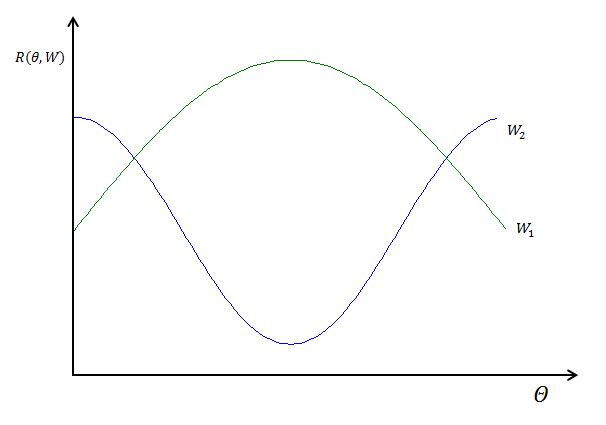
\includegraphics[width=0.7\linewidth]{Figures/Lec21_fig1.jpg}
	\caption[rdr]{Risk v/s $\Theta$ for different estimators}
	\label{fig:Risk function}
\end{figure}
\vspace*{2mm}\newline One way to decide on the best estimator $W^*$ would be to choose the one having smaller peak. One can see that this is equivalent to the minimax estimator (as we are choosing the W with minimum $\underset{\theta}{max}R(\theta,W)$ ).
\vspace*{2mm}\newline Another option is to  choose W that minimizes the area under the R(.,W) function. This is equivalent to the Bayesian estimator.

\section{Notions of Optimality (Rule to compare estimators)}
\begin{enumerate} 
	\item Bayes Risk :
	\newline \hspace*{1cm} Asume a prior probability distribution $\pi$ over the parameter space $\Theta$ is given.
	\newline The bayes risk of W = W(x) is 
	\newline \hspace*{2cm} $B_\pi(W)$ = $\int_{\Theta}^{}R(\theta,W).\pi(\theta)d\theta$
	\newline Any estimator W that minimizes $B_\pi$(.) over all estimators is called a Bayes estimator(denoted by ${W^*}_\pi$) 
	\item Max Risk(No prior necessary): 
	\newline\hspace*{2cm} $\overline{R}$(W) = $\sup_{\theta\in\Theta} R(\theta,W)$
	\newline Estimator minimizing $\overline{R}$(.) are minimax estimators.
\end{enumerate}
\subsection{Bayes Estimators}
Bayes risk under prior $\pi$:
\begin{eqnarray}
B_\pi(W) &=& \int_{\Theta}^{}R(\theta,W)\pi(\theta)d\theta \\
&=& \int_{\Theta}^{}\int_{\mathscr{X}}^{} L(\theta,W(X)).f(x\vert\theta)dx.\pi(\theta)d\theta \\
&=& \int_{\mathscr{X}}^{}\bigg[\int_{\Theta}^{}L(\theta,W(X))\pi(\theta\vert x)d\theta\bigg]m(x)dx
\end{eqnarray}
\newline \hspace*{2cm} where we have used $f(x\vert\theta).\pi(\theta) = \pi(\theta\vert x).m(x) $
\vspace*{5mm}\newline and we have defined
\newline \hspace*{23mm} m(x) $\equiv$ marginal of x
\newline \hspace*{33mm} $ = \int_{\Theta}^{}\pi(\theta').f(x\vert\theta')d\theta' $
\vspace*{3mm}\newline \hspace*{21mm} $\pi(\theta\vert x)\space\equiv$ Posterior density of $\theta$ given x
\newline \hspace*{34mm} $ = \dfrac{\pi(\theta).f(x\vert\theta)}{m(x)} $
\vspace*{5mm}\newline Note that the quantity [.] is a function of only x ( and not $\theta$)
\vspace*{3mm}\newline that implies, to minimize $B_\pi(W)$, we should choose
\newline\hspace*{2cm} $\forall$x $\in$ $\mathscr{X}$ : W(X) $\in$ $argmin_{a\in\mathscr{A}} \int_{\Theta}^{}L(\theta,a)\pi(\theta\vert x)d\theta $
\vspace*{3mm}\newline i.e., a Bayes estimator minimizes the posterior expected loss given the data x.
\vspace*{5mm}
\begin{exmp}[Bayes estimator for square-loss function]
	Let $\Theta\space=\space\mathscr{A}\space=\space\mathbb{R}$
	\newline\hspace*{2cm} $L(\theta,a) = (a-\theta)^2$
	\newline The posterior expected loss is
	\newline \hspace*{2cm} $\int_{\mathbb{R}}^{}(a-\theta)^2\pi(\theta\vert x)dx$
	\newline Then the Bayes estimator is $W(X) = \int_{\Theta}^{}\theta\pi(\theta\vert x)dx $
	\newline i.e., the posterior mean.
\end{exmp}
\begin{exmp}[Bayes estimator for absolute loss function]
	Let $\Theta\space=\space\mathscr{A}\space=\space\mathbb{R}$
	\newline\hspace*{2cm} $L(\theta,a) = |a-\theta|$
	\newline The posterior expected loss is
	\newline \hspace*{2cm} $\int_{\mathbb{R}}^{}|a-\theta|\pi(\theta\vert x)dx$
	\newline Here the Bayes estimator returns $W(X) = MEDIAN(\pi(.\vert x))$
	\begin{proof}
		The posterior expected loss is given by
		\newline $\mathbb{E}\vert x-a \vert$ = $\int_{\mathbb{R}}^{}\vert x-a \vert \pi(\theta\vert x)dx$ = $\int_{-\infty}^{a}-(x-a)\pi(\theta\vert x)dx + \int_{a}^{\infty}(x-a)\pi(\theta\vert x)dx$.
		\newline The bayes estimator is given by 
		\newline\hspace*{2cm} W(x) =  $argmin_a \mathbb{E}\vert x-a \vert$.
		\newline Minimum can be obtained by computing the derivative and equating to 0. 
		\newline\hspace*{2cm} $\dfrac{d}{da}\mathbb{E}\vert x-a \vert = \int_{-\infty}^{a}\pi(\theta\vert x)dx\space - \space \int_{a}^{\infty}\pi(\theta\vert x)dx$
		\newline Equating this equation to zero gives the result as $a = MEDIAN(\pi(.\vert x))$
	\end{proof}
\end{exmp}
\vspace*{3mm} (Similarly a 0-1 loss function returns $W(X) = MODE(\pi(.\vert x))$ )

\subsection{Minimax Estimator}
It turns out that minimax estimation is complicated. The main takeaway here is that the bayes estimator with constant risk over $\Theta$ is minimax.
\begin{defn}  A prior $\pi$ over $\Theta$ is a \textbf{LEAST FAVORABLE PRIOR} if it has the highest bayes risk,i.e
	\newline\hspace*{2cm} $B_{\pi}(W_\pi^*) \geq  B_{\pi\prime}(W_{\pi\prime}^*)$ $\forall$ prior $\pi\prime$ on $\Theta$ .
\end{defn}

\begin{thm}
	Suppose W is the Bayes estimator for some prior $\pi$ over $\Theta$,
	\newline if L($\theta$,W) is a constant $\forall$ $\theta$ $\in$ $\Theta$, then
	\begin{enumerate}
		\item $\pi$ is  a least favorable prior
		\item W is a minimax estimator.
	\end{enumerate}
\end{thm}
\section{Asympotic Evaluation of Estimators}
The goal here is to study what happens to the quality of estimation as the number of samples tend to infinity.
\begin{defn}
	Let $W_n$ $\equiv$ $W_n(X_1,...,X_n)$ for n $\geq$ 1, be a sequence of estimators, for $\theta$, and assuming $X_i$
	$\overset{iid}{\sim}$f(x$\vert \theta$), then $W_n$ is \textbf{CONSISTENT} for estimating $\theta$ if $\forall\theta\in\Theta$, $W_n$ $\overset{P_\theta}{\rightarrow} \theta$.
	\newline i.e $\forall$ $\theta\in\Theta$,$\epsilon >0$, $lim_{n \rightarrow \infty}$P[$\vert$ $W_n$ - $\theta \vert \geq \epsilon$] = 0.
\end{defn}

\textbf{NOTES}
\begin{enumerate}
	\item Consistency is equivalent to convergence to quantity being estimated.
	\item Need convergence in probability $\forall$ $\theta\in\Theta$
\end{enumerate}

Since mean-square convergence implies convergence in probability,
\newline $\forall$ $\theta\in\Theta$, $E_\theta[(W_n-\theta)^2]$ $\rightarrow \infty$  as n $\rightarrow \infty$  is enough to show that \{$W_n$\} is consistent.

\begin{thm}
	If $W_n$ $\equiv$ $W_n(X_1,...,X_n)$ is sequence of estimators such that $\forall$ $\theta$,
	\begin{enumerate}
		\item $lim_{n \rightarrow \infty}var_\theta[W_n]$ = 0
		\item $lim_{n \rightarrow \infty}\mathbb{E}_\theta[W_n]-\theta$ = 0
	\end{enumerate}
	then \{$W_n$\} is consistent.
\end{thm}
\begin{exmp}[Consistency of sample mean]
	Let $X_1,....,X_n$ 	$\overset{iid}{\sim}$ f(x$\vert \theta$),for $\theta$ $\in$ $\Theta$ $\subseteq$ $\mathbb{R}$, and $\forall$ $\theta$ $\in$ $\Theta$, $\mathbb{E}_\theta[\vert X_1\vert]<\infty$,let $W_n$ = $\frac{1}{n}\sum_{i=1}^{n}X_i$; $\forall$ n $\geq$ 1:
	\newline \{$W_n$\} is consistent for estimating $\mathbb{E}_\theta[X]$ since, $\frac{1}{n}\sum_{i=1}^{n}X_i$ $\overset{P_\theta}{\rightarrow}$ $\mathbb{E}_\theta[X_1]$ = g($\theta$), due to the Weak Law of Large Numbers.
\end{exmp}

\subsection{Consistency of Maximum Likelihood Estimator}
\textbf{Recall}  $X_1,....,X_n$ $\overset{iid}{\sim}$ f(x$\vert \theta$),for $\theta\in\Theta\subseteq\mathbb{R}$,
MLE of $\theta$ is $argmax_{\theta \in \Theta} \prod_{i=1}^{n}$f($x_i\vert\theta$) or we can say,
\newline $W_{MLE}$ $\in$ $argmax_{\theta \in \Theta} \sum_{i=1}^{n}$log(f($x_i\vert\theta$)).
\begin{thm}[Consistency of MLE]
	Suppose $X_1,....,X_n$ $\overset{iid}{\sim}$ f(x$\vert \theta$),
	\newline for $\theta\in\Theta\subseteq\mathbb{R}$,and f(x$\vert\theta\in\Theta$) satisfies some regularity conditions, then $\forall \theta \in\Theta$, $W_{MLE}^{(n)}$ $\overset{P_\theta}{\rightarrow}$ $\theta$.
\end{thm}	
	

\end{document}
